\newcommand*{\TeXturedVERSION}{1.5.0} %% TeXtured 2025-08-06
%%%%%%%%%%%%%%%%%%%%%%%%%%%%%%%%%%%%%%%%%%%%%%%%%%%%%%%%%%%%%%%%%%%%%%%
%% NOTE: If you find any issues or have any suggestions, please open %%
%%       an Issue on GitHub: https://github.com/jdujava/TeXtured     %%
%%%%%%%%%%%%%%%%%%%%%%%%%%%%%%%%%%%%%%%%%%%%%%%%%%%%%%%%%%%%%%%%%%%%%%%

%% Enable built-in LaTeX support for PDF/A compliance (must be before `\documentclass`)
\DocumentMetadata{lang=en, pdfversion=1.7, pdfstandard=A-2u}
\input{preamble/pdfA-compliance/glyphtounicode}

%% NOTE: Choose the desirable page layout version (electronic vs print)
\documentclass[12pt,a4paper]{report}                      % single-side (electronic)
% \documentclass[12pt,a4paper,openright,twoside]{report}  % two-sided (for printing)

%% Set some toggle flags to control some of the document properties
\input{preamble/toggles}
% \FANCYfalse % disable some of the more fancy stylistic choices
%% NOTE: Comment out the following lines for the final version
\WIPtrue            % THIS IS A WORK-IN-PROGRESS VERSION
% \EXTRAMARGINtrue  % add extra right margin in WIP version (for notes/corrections)
% \LINKBOXESfalse   % disable reference/link boxes for faster compilations
\CENSORtrue         % THIS IS A CENSORED VERSION

%% Preamble - data, packages, macros, and more
\def\IVEVO{1}
\input{preamble/main}

%% Only uncommented files are included (faster compilation)
%% NOTE: If no files are uncommented, all files are included
\begin{document}
\selectlanguage{english}

\frontmatter
\include{frontmatter/title}
% \include{frontmatter/declaration}
% \include{frontmatter/dedication}
% \include{frontmatter/information}

\contentsandlists

\mainmatter
\chapter{Safety and power precautions}\label{ch:evo-safety}
\textbf{Never power IV-Evo from USB and the vehicle KL30 input at the same time.}
Disconnect the indicator completely from the vehicle harness and any external power source before connecting USB. Do not connect USB while the indicator is installed and connected in the car. The supplied reference excludes warranty and returns for this prohibited use.

Disconnect power before changing connections. Check the connector numbering and the application-specific wiring diagram before applying power.

Protect the front panel from overheating and prolonged direct sunlight. It can exceed 90~$^\circ$C even when switched off. Allow it to cool before touching it to avoid burns.

Configure the indicator while parked. Do not operate the Wi-Fi control panel while driving.

\chapter{Product overview}
IV-Evo is a series of display indicators developed by PHOL-LABS Kft. This manual covers the Golf/Jetta II version; the reference also lists versions for Golf, Jetta, Polo, Audi and LADA vehicles. Check the physical variant before installation.

An ESP32-C3 microcontroller reads vehicle parameters and presents them on the display. Wi-Fi is used for configuration; Bluetooth LE provides telemetry for applications such as gear indication.

Features:

\begin{itemize}
\item 160 by 80 pixels IPS display
\item Tempered glass front panel
\item ESP32C3 MCU
\item Wi-Fi, Bluetooth LE support
\item Lua-configurable and 3rd party apps support
\item Support of raster graphics (JPG, PNG, BMP)
\item Support of simple 3d and 2d animation
\item For Golf, Jetta, Polo and Audi cars and also for LADA cars.
\end{itemize}

\chapter{Package contents}
1x Button-type indicator

1x KF2510 socket with wires


\chapter{Functions and sensor options}
IV-Evo uses selectable applications for the display and sensor scripts for measurement. Configure it over Wi-Fi from a phone or computer. Lua scripts allow custom applications and sensor calibration. Select a sensor script and calibration that match the installed hardware.

Available applications include:
\begin{itemize}
\item IV-Evo  Barometer
\item IV-Evo Thermo
\item IV-Evo Voltmeter
\item IV-Evo Gear indicator
\item IV-Evo Lambda
\item IV-Evo Boost
\item IV-Evo Clock
\end{itemize}
The Check Engine application is also described in this manual.

IV-Evo  Barometer is intended to be working with VAG pressure sensor p.No 03C906051A

IV-Evo Thermo is intended to be working with temperature sensor Ossca 01176 or compatible for Golf 2.

\begin{figure}[htbp]
\centering
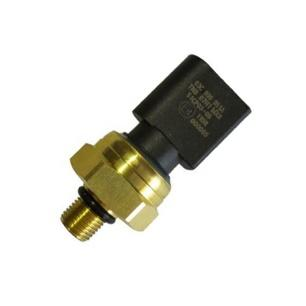
\includegraphics[width=.85\textwidth,height=.60\textheight,keepaspectratio]{figures/ivevo/image21.jpg}
\caption{Sensor reference}
\end{figure}
\begin{figure}[htbp]
\centering
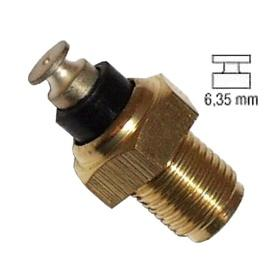
\includegraphics[width=.85\textwidth,height=.60\textheight,keepaspectratio]{figures/ivevo/image19.jpg}
\caption{Sensor reference}
\end{figure}

\chapter{Wi-Fi configuration and wiring}
Wi-Fi is normally off during ordinary operation. Because of the small antenna, keep the phone approximately 10--20~cm from the indicator during configuration.

\begin{enumerate}
\item With USB disconnected, turn on ignition or the intended vehicle supply.
\item Immediately press the rear button. The display should show a QR code.
\item Disable mobile data on the phone. Scan the QR code and connect to the indicator's Wi-Fi network. The documented default password is \texttt{1234567890}.
\item Open \url{http://192.168.4.1} on the connected phone or computer.
\item Select the application and matching sensor, save, then cycle ignition to restart.
\end{enumerate}
If the dashboard is unavailable, move closer and check that the phone remains connected to the indicator's network, even though that network has no Internet access. Retry entering QR-code mode after cycling power.

\begin{figure}[H]
\centering
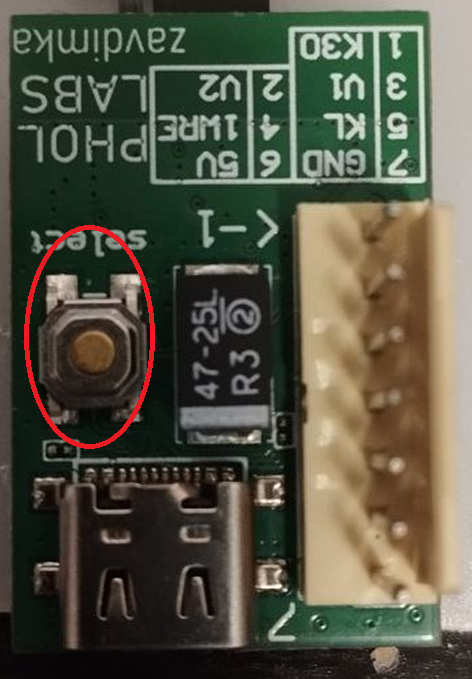
\includegraphics[width=.85\textwidth,height=.60\textheight,keepaspectratio]{figures/ivevo/image11.png}
\caption{IV-Evo reference illustration}
\end{figure}
Rear Wi-Fi boot-mode button.

\section{Common pinout}
\begin{figure}[H]
\centering
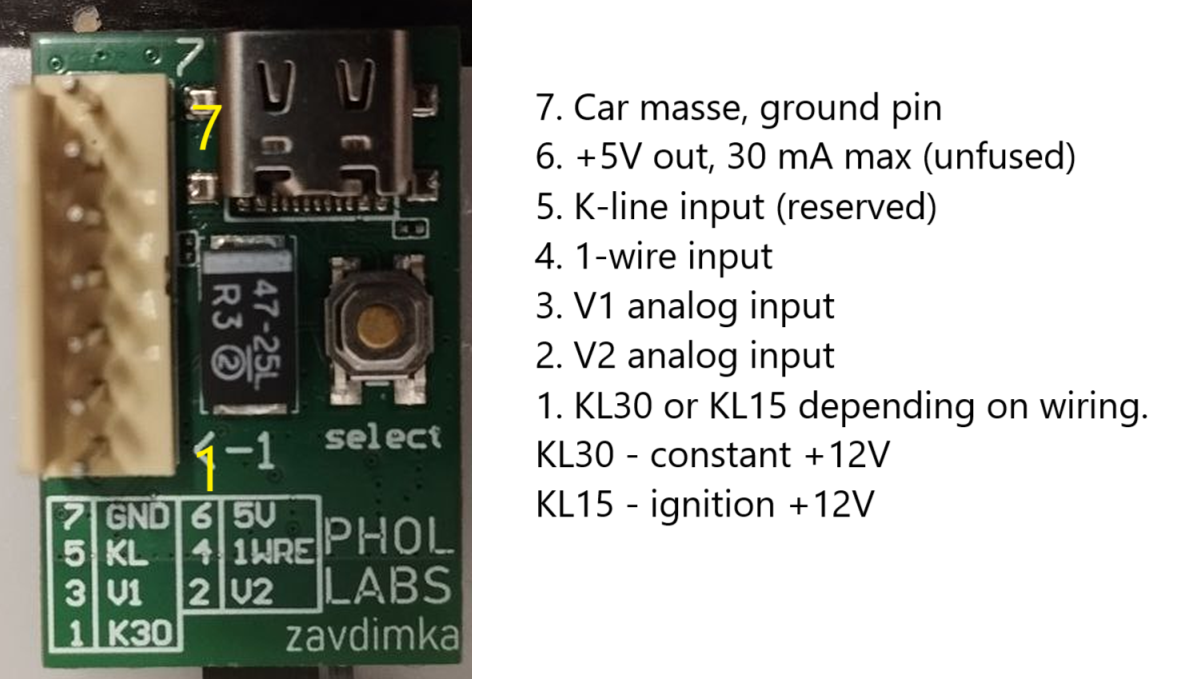
\includegraphics[width=.85\textwidth,height=.60\textheight,keepaspectratio]{figures/ivevo/image20.png}
\caption{Common pinout}
\end{figure}
The device has a seven-pin KF2510 connector. Viewed as in the photograph, the board markings are:
\begin{center}\begin{tabular}{cl}
Pin & Board marking\\\hline
1 & K30 (KL30 power input)\\
2 & V2\\
3 & V1\\
4 & 1WRE (one-wire)\\
5 & KL (K-line, reserved)\\
6 & 5V (+5 V output, 30 mA maximum)\\
7 & GND\\
\end{tabular}\end{center}
Use the numbered pins and the appropriate diagram, not wire colours alone. The supplied voltmeter diagram identifies pin 5 as reserved K-line and specifies a 30 mA maximum for the +5 V output. General analogue input voltage limits are not specified; do not infer them from the pin labels.

USB is intended for initial flashing; subsequent flashing through the web interface is recommended. Disconnect all vehicle wiring before using USB. Follow the instructions supplied with the firmware image: the reference does not specify a recovery sequence or upload menu.

The rear button also interacts with applications and selects the boot mode for initial flashing.

\section{Specific connection schematics}
\clearpage
\subsection{Voltmeter diagram}
\begin{figure}[H]
\centering
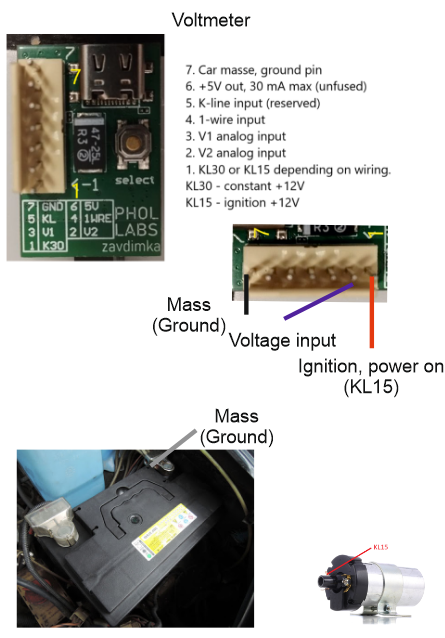
\includegraphics[width=.85\textwidth,height=.60\textheight,keepaspectratio]{figures/ivevo/image5.png}
\caption{Voltmeter diagram}
\end{figure}
\clearpage
\subsection{Gear indicator diagram}
\begin{figure}[H]
\centering
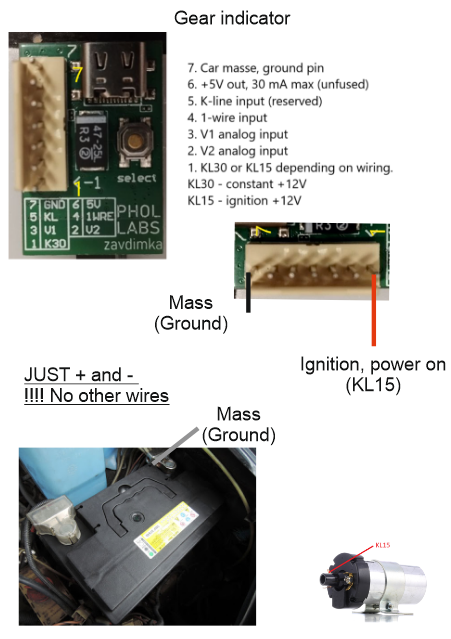
\includegraphics[width=.85\textwidth,height=.60\textheight,keepaspectratio]{figures/ivevo/image6.png}
\caption{Gear indicator diagram}
\end{figure}
\clearpage
\subsection{Barometer diagram}
\begin{figure}[H]
\centering
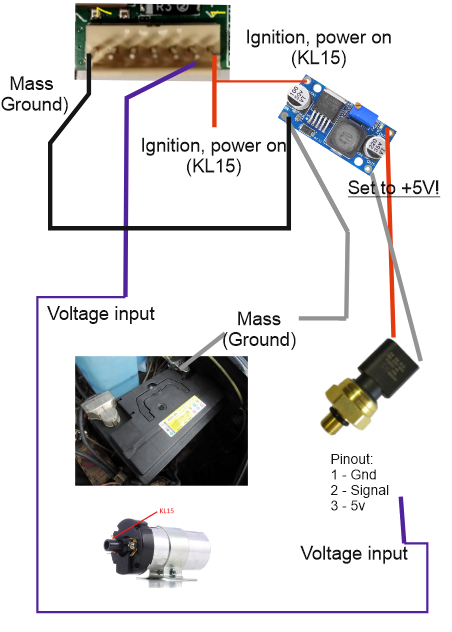
\includegraphics[width=.85\textwidth,height=.60\textheight,keepaspectratio]{figures/ivevo/image1.png}
\caption{Barometer diagram}
\end{figure}
\clearpage
\subsection{Thermometer diagram}
\begin{figure}[H]
\centering
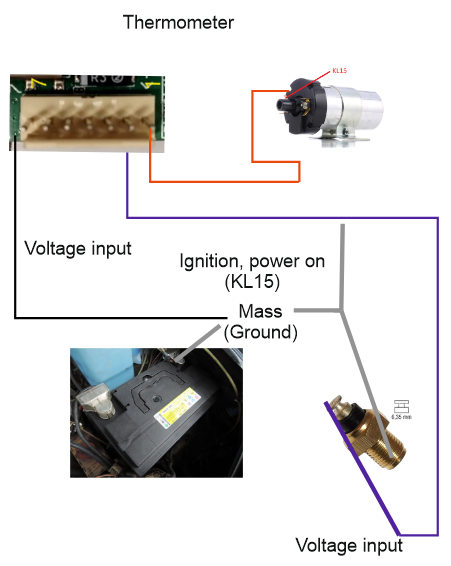
\includegraphics[width=.85\textwidth,height=.60\textheight,keepaspectratio]{figures/ivevo/image13.png}
\caption{Thermometer diagram}
\end{figure}
\clearpage
\subsection{Digital thermometer diagram}
\begin{figure}[H]
\centering
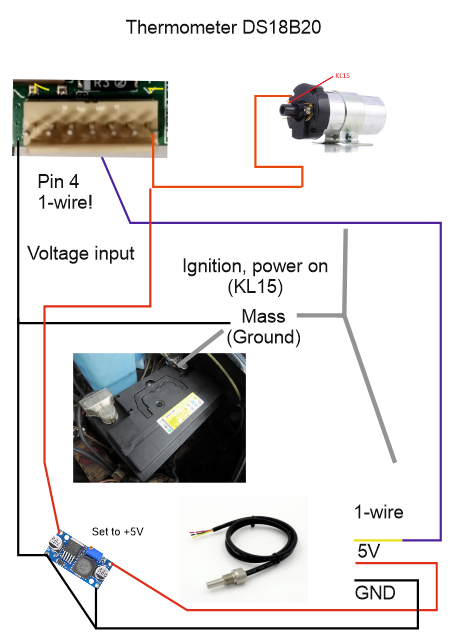
\includegraphics[width=.85\textwidth,height=.60\textheight,keepaspectratio]{figures/ivevo/image8.png}
\caption{Digital thermometer diagram}
\end{figure}
\clearpage
\subsection{Wideband lambda diagram}
\begin{figure}[H]
\centering
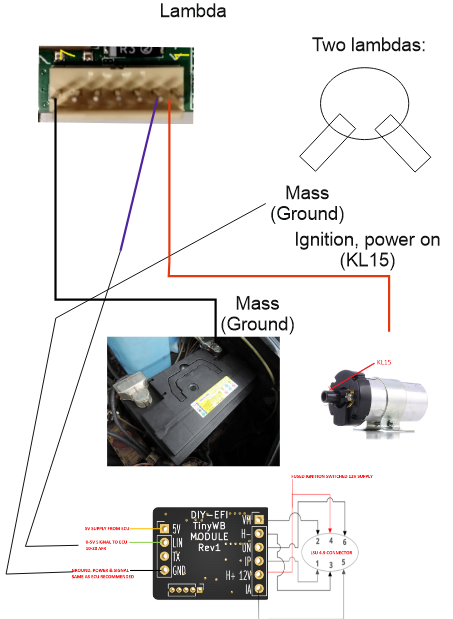
\includegraphics[width=.85\textwidth,height=.60\textheight,keepaspectratio]{figures/ivevo/image3.png}
\caption{Wideband lambda diagram}
\end{figure}
\clearpage
\subsection{Boost indicator diagram}
\begin{figure}[H]
\centering
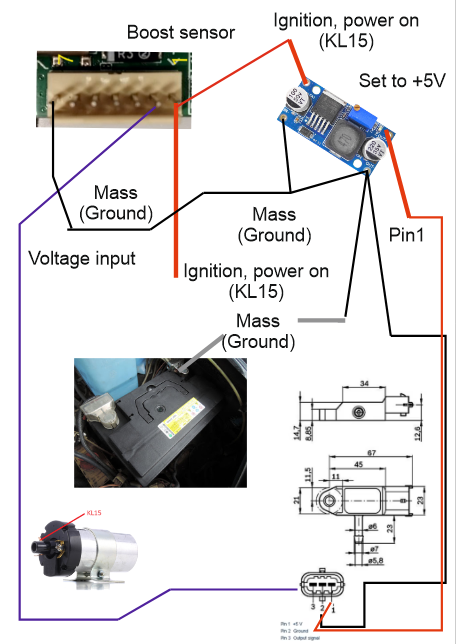
\includegraphics[width=.85\textwidth,height=.60\textheight,keepaspectratio]{figures/ivevo/image17.png}
\caption{Boost indicator diagram}
\end{figure}

\chapter{Applications and calibration}
\section{IV-Evo Voltmeter}
\begin{figure}[htbp]
\centering
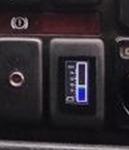
\includegraphics[width=.85\textwidth,height=.60\textheight,keepaspectratio]{figures/ivevo/image16.png}
\caption{IV-Evo Voltmeter}
\end{figure}
\begin{figure}[htbp]
\centering
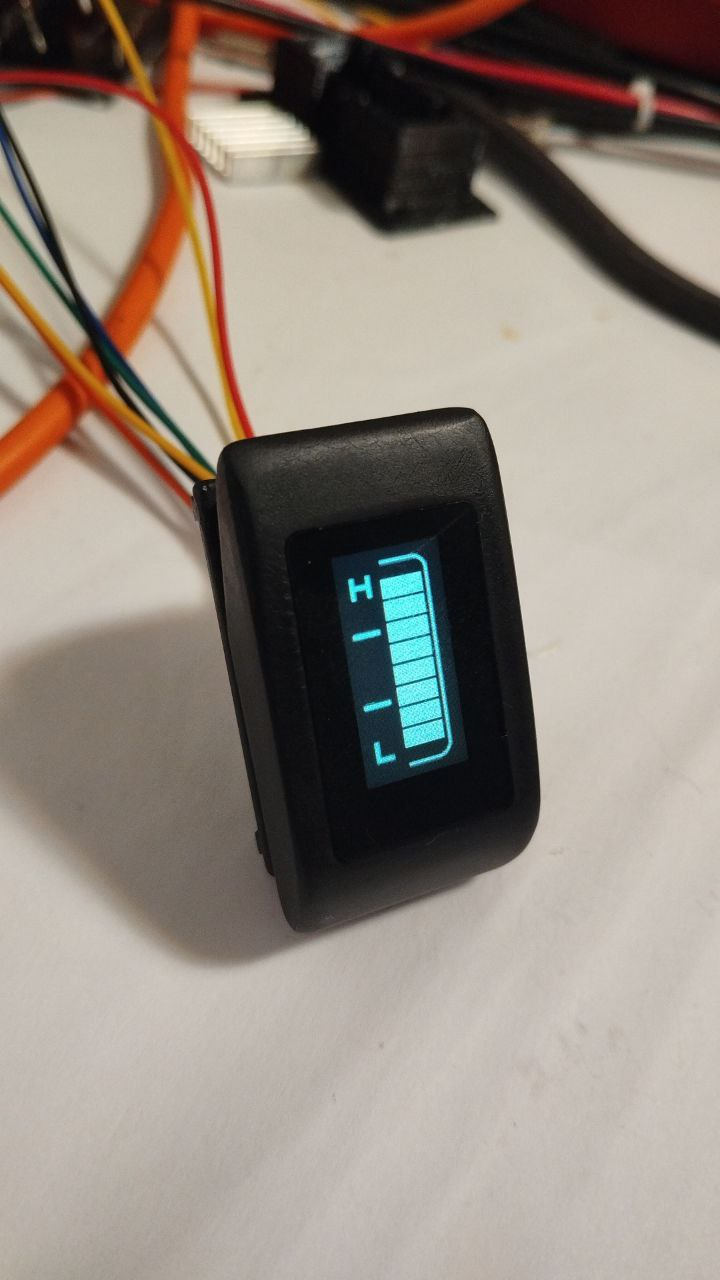
\includegraphics[width=.85\textwidth,height=.60\textheight,keepaspectratio]{figures/ivevo/image15.png}
\caption{IV-Evo Voltmeter}
\end{figure}
\begin{figure}[htbp]
\centering
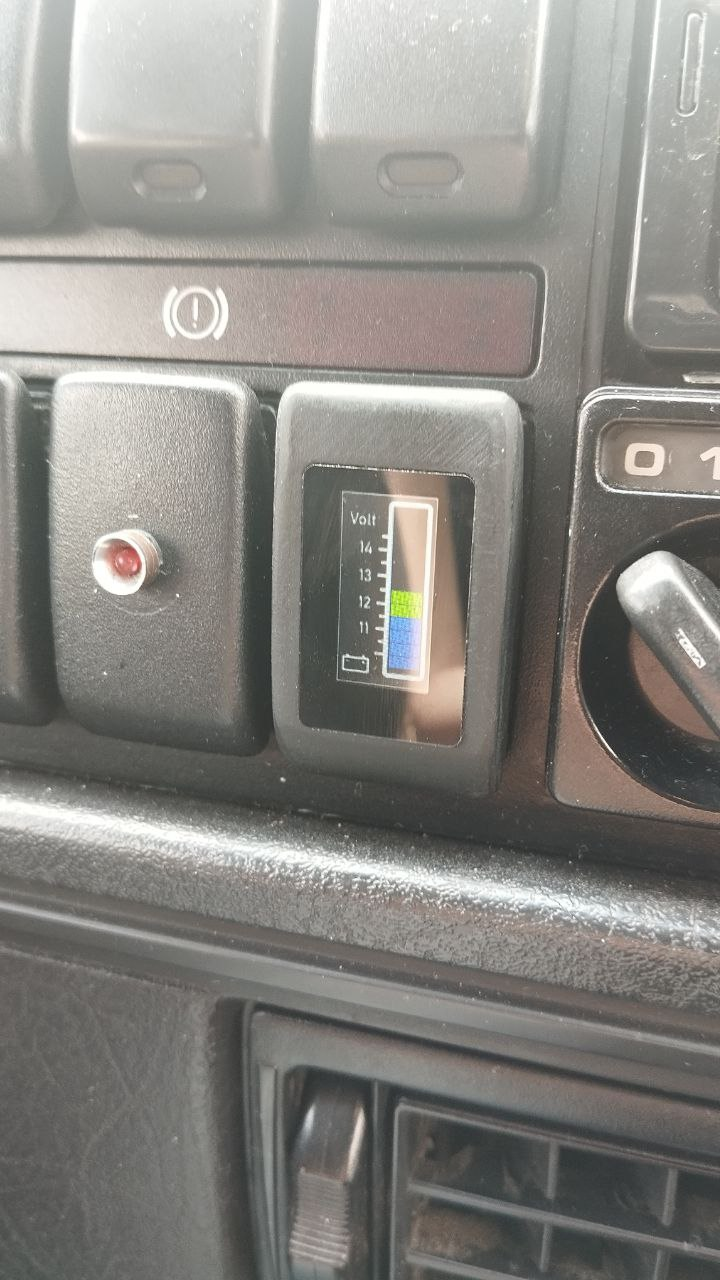
\includegraphics[width=.85\textwidth,height=.60\textheight,keepaspectratio]{figures/ivevo/image2.png}
\caption{IV-Evo Voltmeter}
\end{figure}
IV-Evo voltmeter application type allows you to show the car battery voltage while you are driving.

Applications for the voltmeter:

evo\_v\_l

Displays voltage readings. Includes text voltage and a dedicated background image for voltage monitoring (“battery” icon)

iv\_evo\_v\_t

Displays voltage readings in segments-way like an IV-Nano

\section{IV-Evo  Barometer}
IV-Evo  barometer allows to show car oil pressure while you are driving. Sensor installation is mandatory

IV-Evo  Barometer is intended to be working with VAG pressure sensor p.No 03C906051A

Even though IV-Evo has its own +5V source, it’s still recommended to use external DC/DC for the power.

\section{IV-Evo Thermo}
There are actually two sensor options for IV-Evo Thermo. You can use either NTC or DS18B20 digital sensor.

If thermometer app uses DS18B20 digital sensor to check the temperature in certain location, cables like on the photo are supported, or any other DS18B20 assemblies.

\begin{figure}[htbp]
\centering
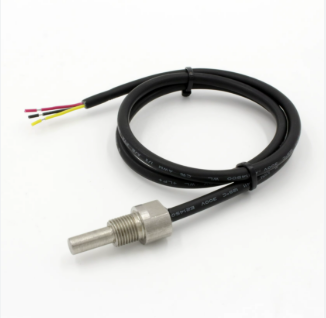
\includegraphics[width=.85\textwidth,height=.60\textheight,keepaspectratio]{figures/ivevo/image14.png}
\caption{IV-Evo Thermo}
\end{figure}
Figure. DS18B20 with bulb and cable

In case of NTC sensor, the following one is recommended:

Ossca 01176

\begin{figure}[htbp]
\centering
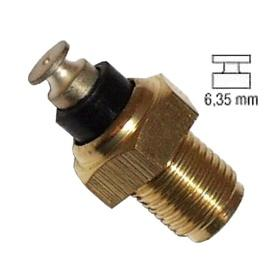
\includegraphics[width=.85\textwidth,height=.60\textheight,keepaspectratio]{figures/ivevo/image19.jpg}
\caption{IV-Evo Thermo}
\end{figure}
On the Ossca sensor, join sensor pins 1 and 2; the NTC resistance is connected to sensor pin 3. These are sensor pin numbers, not the indicator power pins.

\section{IV-Evo Gear indicator}
IV-Evo Gear is a gearbox selected gear indicator, supporting R, 1,2,3,4,5 gears

The idea beyond the indicator is to calculate the gear based on current speed and RPM. Reverse gear is shown if the sensor has positive input on one of inputs.

Device is operated with Bluetooth, and you’ll need Digifiz Next unit in your car for correct operation. Also, speedometer and RPM, as well as gear table should be calibrated to match.

To use IV-Evo Gear, you need to just power it up using pins 1 and 7 (KL30 pin - connect to KL15, ignition power, pin 7 - connect to ground) After that, device will power up and show “-” - meaning that gear is not selected.

Device takes its data from Bluetooth channel from Digifiz Next, so right after the starts its search for Digifiz Next unit.

You’ll need to update your Digifiz Next to a firmware not less than 1.0.14 version, which  introduces BLE streaming of several parameters.

\begin{figure}[htbp]
\centering
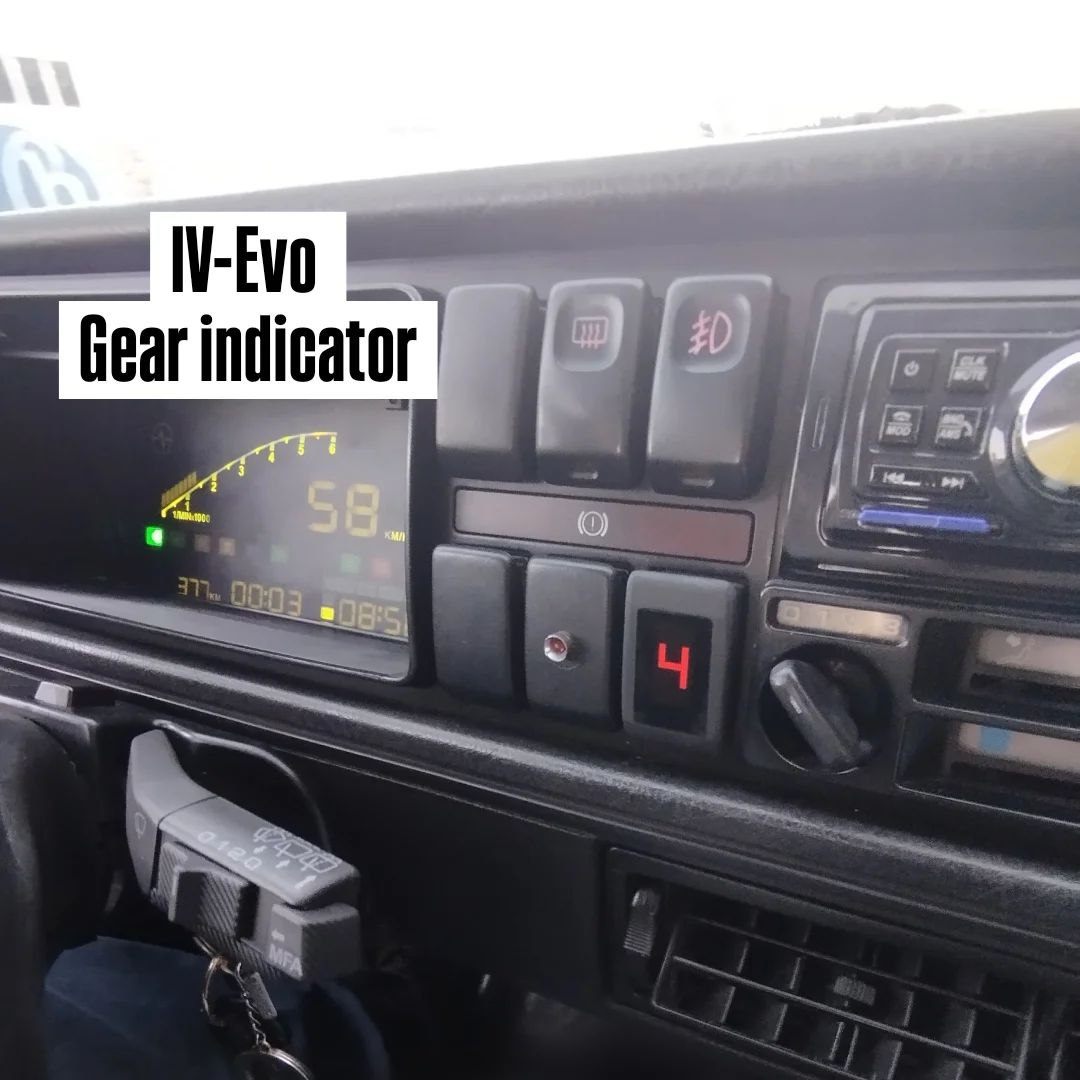
\includegraphics[width=.85\textwidth,height=.60\textheight,keepaspectratio]{figures/ivevo/image18.png}
\caption{IV-Evo Gear indicator}
\end{figure}
\begin{figure}[htbp]
\centering
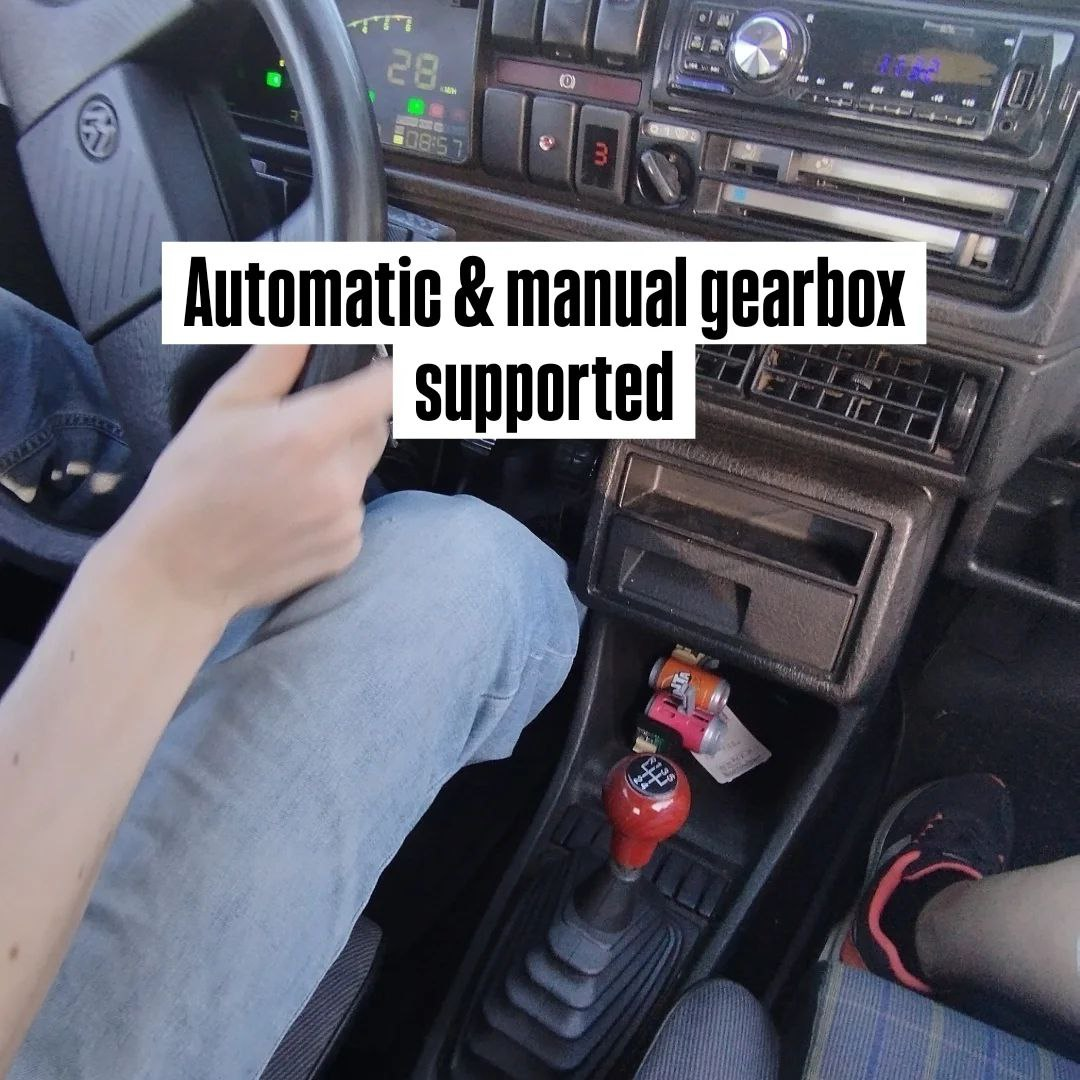
\includegraphics[width=.85\textwidth,height=.60\textheight,keepaspectratio]{figures/ivevo/image10.png}
\caption{IV-Evo Gear indicator}
\end{figure}
Installation guide:

\begin{enumerate}
\item Install Digifiz Next v1.0.14 to your dashboard
\item Connect power +12V KL15 ignition and car masse to pin 1 and pin 7 accordingly
\item Power on in a boot mode(press boot button shortly after turn on) - QR Code will appear. Scan it from you phone and connect to the dashboard.
\item Select application and sensor - “iv\_gear” and “volts1”, save selection
\item Restart by ignition off and on
\item Preliminary installation is complete!
\end{enumerate}
After that, you’ll need to perform a tuning of parameters on Digifiz Next cluster Wi-Fi control panel.

\begin{enumerate}
\item First of all, calibrate your speed using GPS speed from your phone, use 80--100 km/h as a reference only where lawful and safe, with a passenger recording readings.
\end{enumerate}
The parameter for speed calibration is on the Settings page.

\begin{enumerate}
\item After that, calibrate RPM setting by using the same settings page. The source mentions calibration values 1500, 3000 and 400 but does not define their units or map them unambiguously to engines. Use the Digifiz Next instructions for the actual engine rather than selecting an arbitrary value. The speed, RPM and gear table must all match the vehicle.
\end{enumerate}
\section{IV-Evo Lambda}
\begin{figure}[htbp]
\centering
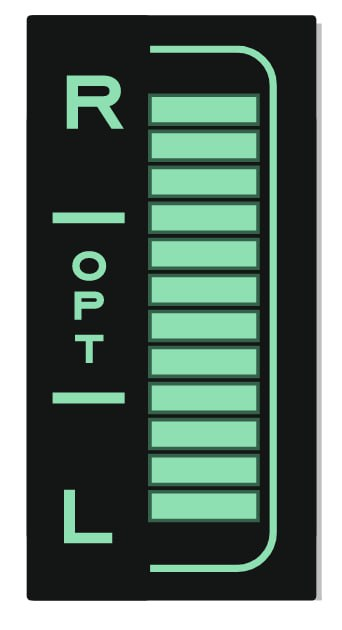
\includegraphics[width=.85\textwidth,height=.60\textheight,keepaspectratio]{figures/ivevo/image7.png}
\caption{IV-Evo Lambda}
\end{figure}
For IV-Evo Lambda the connection is somewhat more complicated.

It is important that connection to stock Golf 2 lambda sensor is not possible

Lambda sensor measurement should be done with 2 lambda sensors installed in the car.

There are two types of Lambda sensors:

Narrowband Oxygen Sensor:

\begin{itemize}
\item Operation: Measures only whether the air-fuel mixture is rich or lean.
\item Output: Produces a voltage between 0.1V (lean) and 0.9V (rich), without detailed information on the exact air-fuel ratio.
\item Use: Common in older vehicles for basic emissions control.
\end{itemize}
Wideband Oxygen Sensor:

\begin{itemize}
\item Operation: Provides precise measurements of the actual air-fuel ratio over a wide range, not just rich or lean.
\item Output: Delivers a linear signal, giving the engine control unit detailed feedback to optimize fuel injection.
\item Use: Found in modern vehicles for more accurate fuel management and emissions control.
\end{itemize}
The problem is that narrowband sensors are not applicable for most of custom engines and carburetors, only wideband ones. And they are more advanced, require more control operations. The indicator itself cannot control wideband sensor, and works directly only with narrowband sensors(needs to be calibrated though)

However, installation of wideband sensor is possible and recommended. For wideband sensor we do recommend Bosch LSU 4.9 sensor, which should be accompanied with supported wideband controller:

\begin{itemize}
\item SLC Free
\item DIY-EFI TinyWB Wideband controller
\item Sigma Lambda Controller Free 2
\item rusEFI wideband lambda
\item Others
\end{itemize}
After buying such wideband controller please connect it according to its diagram to LSU 4.9 and use analog output (typically, 0-5V, 0.5-4.5 or even 0-1V output) for connection to the IV-Indicator Lambda. Below, on connection diagrams, you can find an example connection.

\section{IV-Evo Check Engine}
\begin{figure}[htbp]
\centering
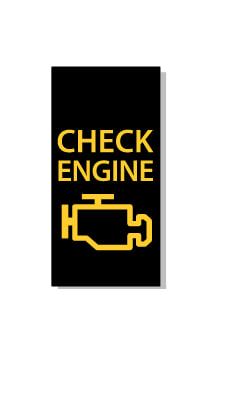
\includegraphics[width=.85\textwidth,height=.60\textheight,keepaspectratio]{figures/ivevo/image4.png}
\caption{IV-Evo Check Engine}
\end{figure}
IV Evo Check Engine is a check engine indicator for your car. It displays “Check engine” or empty screen depending on pin 2 - V2, state. If it’s 12V - Check Engine is displayed, if 0V - nothing is displayed.

\section{IV-Evo Boost}
IV-Evo Boost displays boost pressure while driving. Sensor installation is mandatory

The following sensor is recommended for the installation:

\begin{figure}[htbp]
\centering
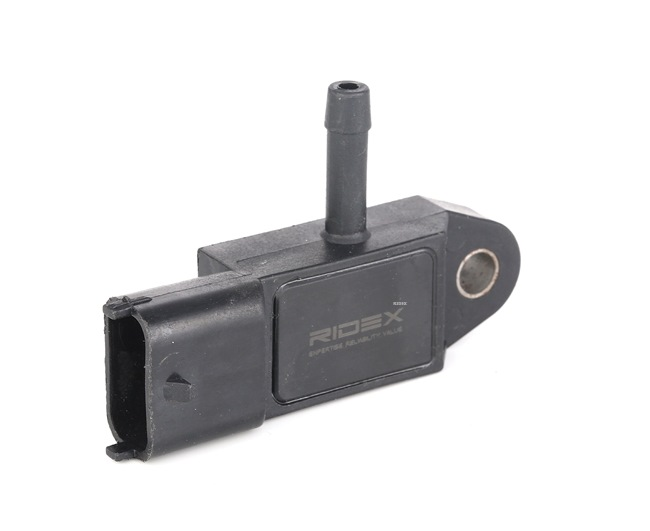
\includegraphics[width=.85\textwidth,height=.60\textheight,keepaspectratio]{figures/ivevo/image9.png}
\caption{IV-Evo Boost}
\end{figure}
Boost sensor characteristics:

\begin{itemize}
\item Number of pins:3
\item Power voltage: +5 V
\item Number of mounting bores:1
\item Pressure from [kPA]:20
\item Pressure to [kPA]:250
\item Nominal sensor output voltage: +1.8V
\end{itemize}
\section{IV-Evo Clock}
\begin{figure}[htbp]
\centering
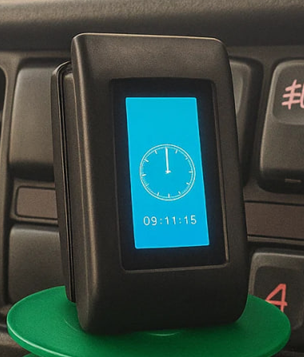
\includegraphics[width=.85\textwidth,height=.60\textheight,keepaspectratio]{figures/ivevo/image12.png}
\caption{IV-Evo Clock}
\end{figure}
IV-Evo clock is an example app which works like a system clock of the indicator. Works like a bootstrap app for the indicator. However, the time is not saved on boot, so it only acts as trip time indicator in that case.


\section{Calibration limits in the reference}
The boost sensor description does not provide a full voltage-to-pressure transfer function or identify the pressure at its nominal +1.8 V output. Confirm the exact sensor and calibration curve before setting the scale. The reference gives no general enclosure ingress rating, operating temperature range or supply voltage tolerance; do not assume Nano specifications apply.

\appendix
\chapter{Lua API reference}
This document describes the Lua runtime model used by the firmware and the currently exposed Lua namespaces (modules) implemented in C.

The goal is to help you write two Lua files:

\begin{itemize}
\item App script (app.lua) with UI logic (drawing on display, handling loop, etc.).
\item Sensor script (sensor/*.lua) that provides measured values through sensor.get(index).
\end{itemize}
\section{Runtime model}
\subsection{App contract}
Each app file returns a table (commonly M) with callbacks:

\begin{itemize}
\item M.loop() required
\item M.init() optional
\item M.event(event\_type) optional
\item M.cleanup() optional
\end{itemize}
The firmware loads your app, stores these callbacks, and executes loop() repeatedly. If loop is missing, the app is rejected. On runtime errors, firmware can switch to a fallback app.

\subsection{Sensor contract}
Sensor Lua file should return a table named sensor with:

\begin{itemize}
\item sensor.get(index) returning a numeric value.
\end{itemize}
The firmware loads the sensor script and stores it globally as sensor, then app scripts call sensor.get(...).

\subsection{Globals provided by firmware}
\begin{itemize}
\item apppath — path to current app folder (useful for loading assets/fonts relative to app location).
\item sensor — table returned by active sensor script.
\end{itemize}
\section{Lua namespaces (modules)}
The firmware registers the following Lua modules:

\begin{itemize}
\item display
\item system
\item onewire
\item nvs
\item ble
\end{itemize}
Load them in Lua with require("module") (or via pcall(require, "module") for optional usage).

\section{API reference}
\section{display}
\subsection{Resource management}
\begin{itemize}
\item display.loadimg(path) -> img\_handle|nil
\end{itemize}
\begin{itemize}
\item Decodes image and returns handle (integer-like pointer).
\end{itemize}
\begin{itemize}
\item display.loadfont(path) -> font\_handle|nil
\item display.free(handle)
\end{itemize}
\begin{itemize}
\item Frees image/font allocated by loadimg / loadfont.
\end{itemize}
\subsection{Frame control}
\begin{itemize}
\item display.fill(color)
\end{itemize}
\begin{itemize}
\item Fills entire screen.
\end{itemize}
\begin{itemize}
\item display.update()
\end{itemize}
\begin{itemize}
\item Flushes frame and clears screen to black afterwards.
\end{itemize}
\subsection{Drawing primitives}
\begin{itemize}
\item display.drawimg(img, x, y)
\item display.string(font, x, y, text, color)
\item display.fillrect(x, y, width, height, color)
\item display.drawline(x1, y1, x2, y2, color)
\item display.drawcircle(x, y, r, color)
\item display.drawfillcircle(x, y, r, color)
\item display.drawroundrect(x1, y1, x2, y2, r, color)
\item display.drawarrow(x0, y0, x1, y1, w, color)
\item display.drawfillarrow(x0, y0, x1, y1, w, color)
\item display.drawpolygon(\{x1, y1, x2, y2, ...\}, color)
\end{itemize}
\begin{itemize}
\item Even count of coordinates required (at least 4 elements).
\end{itemize}
\subsection{Color constants}
\begin{itemize}
\item display.RED
\item display.GREEN
\item display.BLUE
\item display.WHITE
\item display.BLACK
\item display.YELLOW
\item display.CYAN
\item display.PURPLE
\item display.GRAY
\end{itemize}
\section{system}
\begin{itemize}
\item system.delay(ms)
\item system.backlight(level)
\item system.V2\_pullup(enable)
\item system.out5V(enable)
\item system.keys() -> int
\item system.adc\_ch(channel) -> number
\item system.get\_time() -> hour, minute, second
\item system.config\_sleep(enable)
\end{itemize}
\section{onewire}
\begin{itemize}
\item onewire.scan18b20() -> count
\item onewire.read18b20(index) -> temperature\_c
\end{itemize}
\section{nvs}
Namespace is backed by NVS partition namespace app.

\begin{itemize}
\item nvs.get(key) -> string|nil
\item nvs.push(key, value\_string) -> boolean
\end{itemize}
\section{ble}
\begin{itemize}
\item ble.init() -> true
\item ble.get\_telemetry() -> rpm, speed, gear
\end{itemize}
\section{Example \#1 — Simple voltmeter app}
The coordinates below fit the 160 by 80 pixel screen, and the bar width is clamped.
Below is a minimal app using the same style as existing voltmeter apps (sensor.get(1), font draw, cleanup).

\begin{verbatim}
local M = {}
local font = display.loadfont(apppath .. "/../fonts/H24XB.FNT")

local function read_voltage()
return sensor.get(1)
end

function M.loop()
local v = read_voltage()
display.fill(display.BLACK)
display.string(font, 10, 30,
    string.format("%2.1f V", v), display.WHITE)
display.fillrect(10, 60,
    math.max(0, math.min(140, math.floor((v - 9.5) * 12))),
    8, display.GREEN)
display.update()
end

function M.cleanup()
display.free(font)
end

return M
\end{verbatim}
Notes:

\begin{itemize}
\item display.update() is called once per frame.
\item cleanup() should free loaded resources.
\item Clamp bar calculations in production code (existing apps clamp values to display range).
\end{itemize}
\section{Example \#2 — Sensor Lua script (NTC-like)}
This script demonstrates reading ADC, enabling pull-up rail, smoothing, and returning processed value.

\begin{verbatim}
sensor = {}

local filt = 0.0

function sensor.get(i)
i = i or 0
system.V2_pullup(1)

local raw = system.adc_ch(i)
filt = filt + (raw - filt) / 10.0

-- Example transform (replace with your real calibration/math):
local value = filt * 1.0
return value
end

return sensor
\end{verbatim}
Notes:

\begin{itemize}
\item Keep sensor.get(i) fast; it is called from app loops.
\item You can store calibration in NVS (for example, via nvs.get("key") and tonumber(...)).
\end{itemize}
\section{Practical tips}
\begin{itemize}
\item Use pcall(require, "nvs") when NVS access is optional.
\item Build paths from apppath for portable assets (apppath .. "image.jpg", apppath .. "/../fonts/...").
\item Always free display.loadimg / display.loadfont handles in cleanup().
\item If using DS18B20, call onewire.scan18b20() once and onewire.read18b20(index) in loop.
\end{itemize}

\end{document}
